\chapter{Luminometer Calibration}
\label{ch3}

\section{Van Der Meer Method}

The Van Der Meer (vdM) scan let us obtain the value of $\sigma_{visible}$ using different luminometers. For this case the detector of interest is the pixel detector with which are going to obtain a calibration of the luminosity using the vdM scan in combination with the PCC method. The scan consist on separating particle the beams from each other between the X and Y axis by $\Delta X$ and $\Delta Y$ values moving them and recording values of luminosity independently, when the scan on X and scan on Y are imposed over each other we said that they're on head on giving the maximum value of luminosity. Usually a single gaussian fit is used to obtain beam overlap widths also denoted as $\Sigma_{x}$ and $\Sigma_{y}$, other fit models may be used like the doble gaussian depending on the quality of the fit \cite{Vdm}

\begin{figure}[h]
    \centering
    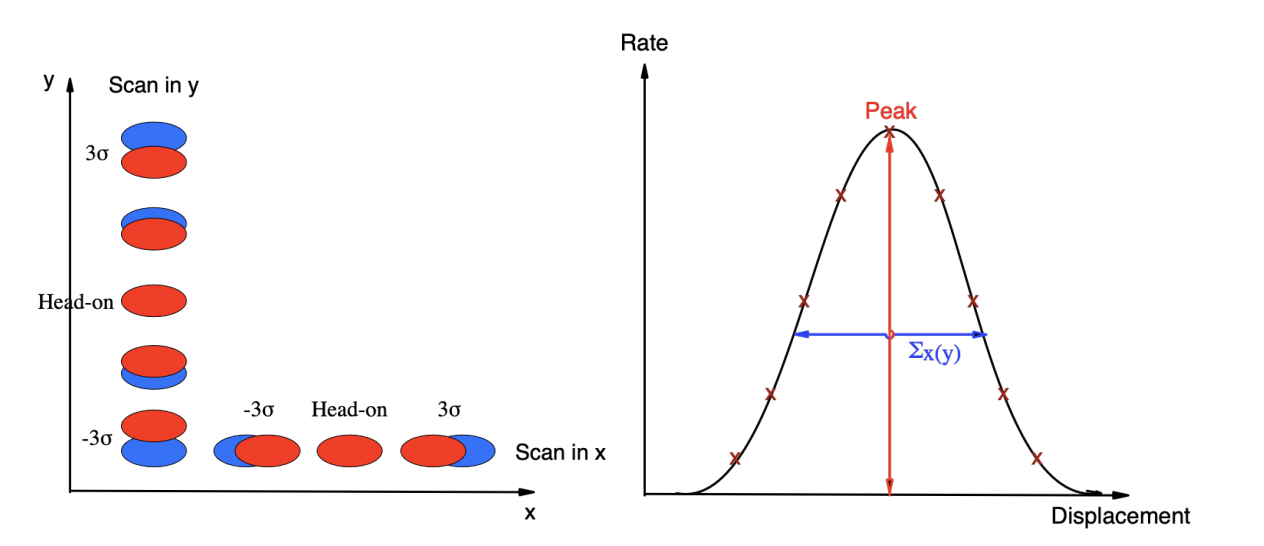
\includegraphics[width=1\textwidth]{vdm1.png}
    \caption{The vdm scan on the left showing the beams for X and Y. On the right a curve of the different values of rate for the beams displacement, the peak occurs during the head on part.}
    \label{fig:vdm1}
\end{figure}


For obtaining the important parameters on the vdm scan we return to the equation (1.2) and apply it to and individual bunch crossing, the values of N1 and N2 being the number of protons colliding can be obtained since is a known quantity from the experiment, the frequency f is also a known quantity, the frequency of the LHC which is 11,245 kHz but the proton densities $\rho_{1}$ and $\rho{2}$ are more difficult to obtain, this is were the vdM scan help us to measure integral over the bunch proton densities. The luminosity integral evaluated with the beams separated by a distance $\Delta_{x}$ and $\Delta_{y}$ can take the form of: 

\begin{equation}
 L(\Delta x, \Delta Y) = N_{1} N_{2} f  \int \int \rho_{1}(x,y)\rho_{2}(x+\Delta x, y+\Delta y) dxdy 
\end{equation}

Because of the scan method is it assumed that the two bunches of proton densities are factorizable since they act independently between each other so we can turn the right part of (3.1) into two integrals:

 \begin{equation}
N_{1} N_{2} f  \int \int \rho_{1}(x,y)\rho_{2}(x+\Delta x, y+\Delta y) dxdy   = N_{1} N_{2} f (\int \rho_{1}(x)\rho_{2}(x + \Delta x) dx) (\int \rho_{1}(y) \rho_{2}(y + \Delta y) dy)
\end{equation}

Integrating both sides on $\Delta y$ and using in combination with (3.1) while we fix $\Delta x_{0}$ = 0 and $\Delta y_{0}$ = 0 as the head on point,  we obtain:
 
 \begin{equation}
N_{1} N_{2} f \int \rho_{1}(x) \rho_{2}(x + \Delta x_{0}) dx = \int L (\Delta x_{0}, d\Delta y) d(\Delta y)
\end{equation}

A similar result is obtained when we integrate both sides for $\Delta x$ using this and combining equation (3.1), (3.2) and (3.3) we can obtain that 

\begin{equation}
N_{1} N_{2} f \int \rho_{1}(x) \rho_{2}(x + \Delta x_{0}) dx = \frac{L (\Delta X_{0}, \Delta y_{0})}{\int L(\Delta x_{0}, \Delta y) d(\Delta y)}
\end{equation}

Similarly to the previous step we can obtain the value of the other factor of (3.2) with an analogous process. The integrals resulting on the right side can be evaluated by evaluated by obtaining the rate in function of the beam-beam separation which are $\Delta x$ and $\Delta y$  this because the luminosity has a linear relationship with the rate. The Luminosity can be expresed on terms of the rate during the head on positions, R(\Delta_{x0}, \Delta_{y0}) like in the equation (3.5)

\begin{equation}
L(\Delta x, \Delta y) = N_{1} N_{2} f \frac{2R(\Delta x_{0}, \Delta y_{0}){\int L(\Delta x_{0}, \Delta y) d(\Delta y) \int L(\Delta x, \Delta y_{0}) d(\Delta x)}}
\end{equation}

Here the luminosity is replaced by the rate R, it is convenient to write this integral in terms of the convoluted beam widths which are denoted by $\Sigma_{x}$ and $\Sigma_{Y}$, this convoluted widths are defined by: 

\begin{equation}
\Sigma_{x} = \frac{1}{2 \pi} \frac{\int R(\Delta x, \Delta y_{0}) d(\Delta x) )}{R(\Delta x_{0}, \Delta y_{0})}
\end{equation}

For $\Sigma_{y}$ the result is analogous. With (3.6) we can write (3.5) in a different manner:

\begin{equation}
L(\Delta x, \Delta y) = \frac{N_{1}N_{2}f}{2 \pi \Sigma_{x} \Sigma_{y}}
\end{equation}  

This in combination with (1.4) make us possible to obtain the following expression for the visible cross section

\begin{equation}
\sigma_{vis} = \frac{2 \pi \Sigma_{x} \Sigma_{y} R(\Delta x_{0}, \Delta y_{0})}{N_{1} N_{2}f}
\end{equation}

This makes possible obtain $\sigma_{vis}$ only by experiment since all of the right values can be obtained via the experiment, the maximum rate R($\Delta x_{0}$, $\Delta y_{0}$) is obtained at the maximum PCC obtained during the vdm scan, this means during the head-on process, while the $\Sigma_{x}$ and $\Sigma_{y}$ are obtained with the information of the fit model. 

This calculations are done on several Bunch Cross Identifier which so you obtain several values of $\simga_{vis}$ and then they are weight averaged according to the uncertainties in order to obtain $\sigma_{vis}$ for the scan. 

\section{Datasets}

The data on the CMS is a complex set of inter-dependent workflows made in a way that assure the full physics exploitation of the CMS detector potential and the collisions delivered by the LHC, this data provides analyses with reconstructed collision events from the experiment and are designed to use the CMS computing resources efficiently. This stream of events is organized into datasets according to the results of the High Level Trigger (HLT) which defines primary datasets since they are defined by the paths of the HLT. The design of the primary datasets is centered around candidates for particles that are reconstructed on the final state by the hLT and follows the principle of grouping together events with similar physics content.    \cite{datasets1}

The datasets used for the obtention of the $\sigma_{visible}$ for 2024 were the ones from the Fill 9639 which is divided in 3 blocks, a fill is a process that generates beams for the LHC this tipycally involves particles around the number of $10^{14}$ that are grouped in bunches that form the proton beam. This is what we use the bcid number to identify this bunches, there are a total of 3564 bunches that are empty or filled depending on the fill all of this part of the LHC bunch train. For this fill in the calibration the bcids of relevance were a total of 12 which are identified by the numbers: 303, 324, 345, 506, 527, 822, 1081, 1102, 1397, 2000, 2965, 3123. 

In the case for our datasets each bcid is processed by the CMS collaboration to enable cluster reconstruction resulting in the ALCARECO datasets that contain a module collection and their number of cluster per event in CMSWW format. This samples are processed using the CMSWW software to extract the clusters per module to obtain the dataset in the ROOT format. ROOT is a software framework born at CERN It is open source and used for high energy physics to analyze data while providing packages for storage, processing and visualization while minimizes the computing resources needed. 

The root format saves the data in form of TTrees which behaves like an array of data structure and storage data. This tree consist on branches and leaves, a branch is a list of independent columns that can contain values of any fundamental type and are represented by TBranch. While the leaves represented by TLeaf give access to actual data in difference to the TBranch which represent a structure. After the datasets are processed, the rates of the Pixel detector were stored each 1.32 seconds periods called NB4 this to make an average of clusters and the number of events that fall into that time span. 

This dataset were first processed by the CMS collaboration enabling a cluster reconstruction resulting in the ALCARECO datasets getting a lot of root files for each of the different zero bias streams that were the starting point of this analysis. 

After this the data then was processed again to obtain a hd5file a format that can supports n-dimensional datasets and facilitates the reading of the datasets, this hd5 files contained relevant information about the root files like the average rate per NB4, this was made for each of the files for almost all of the available streams excluding two of them that were not ready by the moment (the ones that were identified by ZB21 and ZB28) after one stream got all of his files processed into an hd5 file they were converged into a single file containing relevant information for all the stream, once all of the files in all of the data streams were processed into hd5 files a single hd5file was made containing all of the information about the streams also a single csv file was made containing only the average rate file per NB4 for each of the bcids.  

This scans were analyzed using the vdM framework, a CMS tool to obtain different parameters using a fit model on the vdM scans, this framework read hd5 files and with a set of instructions the value of $\sigma_{visible}$ can be obtained. 
 
\section{Scans}

For the calibration of 2024 in the LHC fill 9639 during may 15 to may 16 at collision proton proton with a energy of 13.6 TeV, the vdm scans were made there were a total of 5 vdm X and vdm Y scans and 2 beam img X and beam img Y and the Super Separation period which is a scan used to obtain a background estimation, this were the scans used on this analysis to compute the value of $\sigma_{visible}$. The figure (3.x) shows a DOROS image of the fill and all the scans that were made during that period of time. 

\begin{figure}[h]
    \centering
    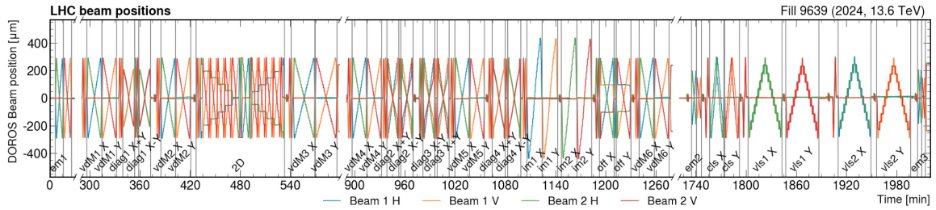
\includegraphics[width=1\textwidth]{scans.png}
    \caption[Doros for fill 9639]{DOROS beam position during LHC Fill 9639 for the vdM scans. Horizontal and vertical beams are shown over time}
    \label{fig:scans}
\end{figure}

The 5 vdm scans vdM1, vdM2..., vdM5 are the scans usually used in the calibration to compute $\sigma_{visible}$ two beams are separated the transverse bunch size and then scanned across one another in sequence of 25 steps with 30 seconds per step. The beam imaging scan is kept on a nominal position while the other is separated and scanned in 19 steps, the scan is performed first in the X direction and then in the Y direction. The Super Separation scans separates the beams a distance were the overlap of the beams is negligible, the minimum possible.

\section{Background Estimation}

The background estimation were obtained using the 5 Super Separation scans, the time on which this super separations were used was on UNIX time, this time can be defined as a system for tracking a point in time as the number of seconds that have happened since January 1 at 00:00 in universal time (UTC). Each of these super separations lasted a total of 5 minutes in the following table we got more information about the start and ending of the scans. 

\begin{table} [H]
\begin{center}
\caption{Super Separation Period time}
\begin{tabular}{|c c c|} 
 \hline
 Scan & Time Start & Time End  \\ [0.5ex] 
 \hline\hline
 SS1 & 1715883182 & 1715883481  \\ 
 \hline
 SS2 & 1715902185 & 1715902484  \\
 \hline
 SS3 & 1715919164 & 1715919463 \\
 \hline
 SS6 & 1715943045 & 1715943343  \\
 \hline
 SS5 & 1715987303 & 1715987602  \\ [1.0ex]
 \hline
\end{tabular}
\end{center}
\end{table}

The data of this scans were processed and analyzed, in the following image we show the mean value of the PCC rates during the Super Separation period scan in one bcid.

\begin{figure}[H]
    \centering
    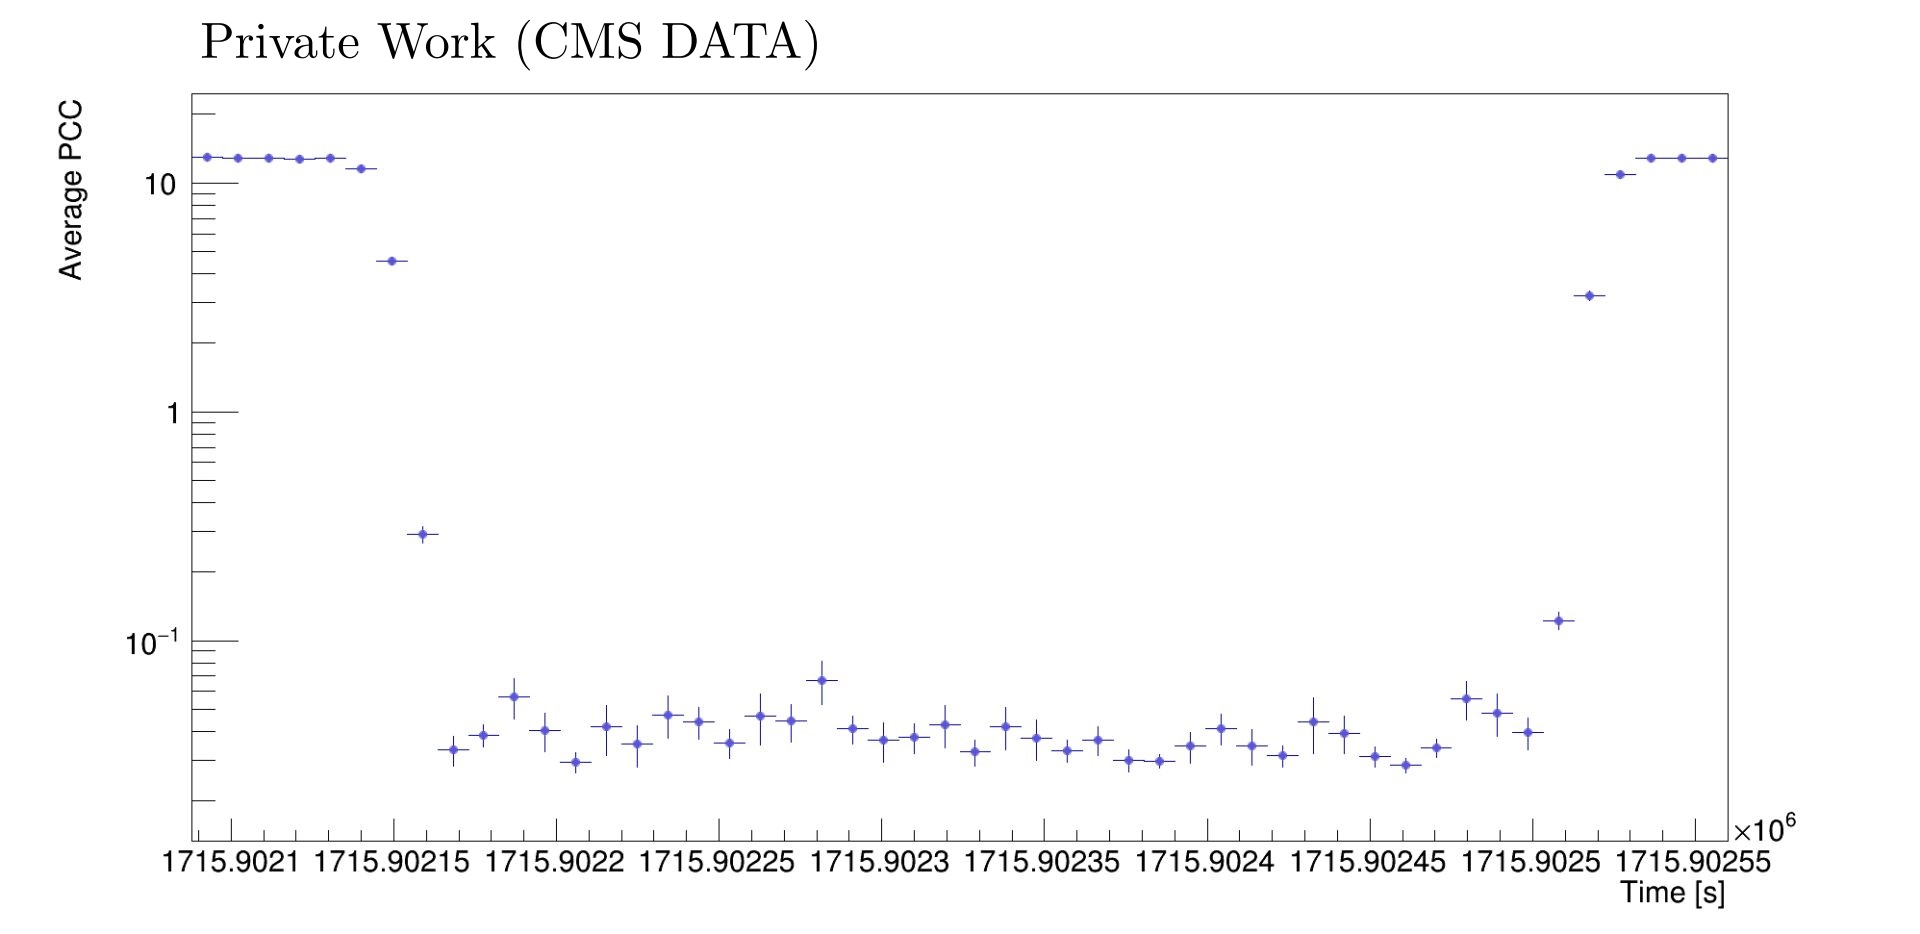
\includegraphics[width=1\textwidth]{SS1.jpeg}
    \caption{Mean rates during the second super separation scan}
    \label{fig:SS1}
\end{figure}

The reason why the background estimation is obtained during the super separation (SS) process, It's because the SS scan separates the beams so they shouldn't be colliding the expected value on the rate is expected to be a rate associated with the background, this was obtained checking the mean values for each bcid for all the entries of pcc rates for each of the 5 periods of super separation, the following image illustrate a case for one SS period and bcid 50x:

\begin{figure}[H]
    \centering
    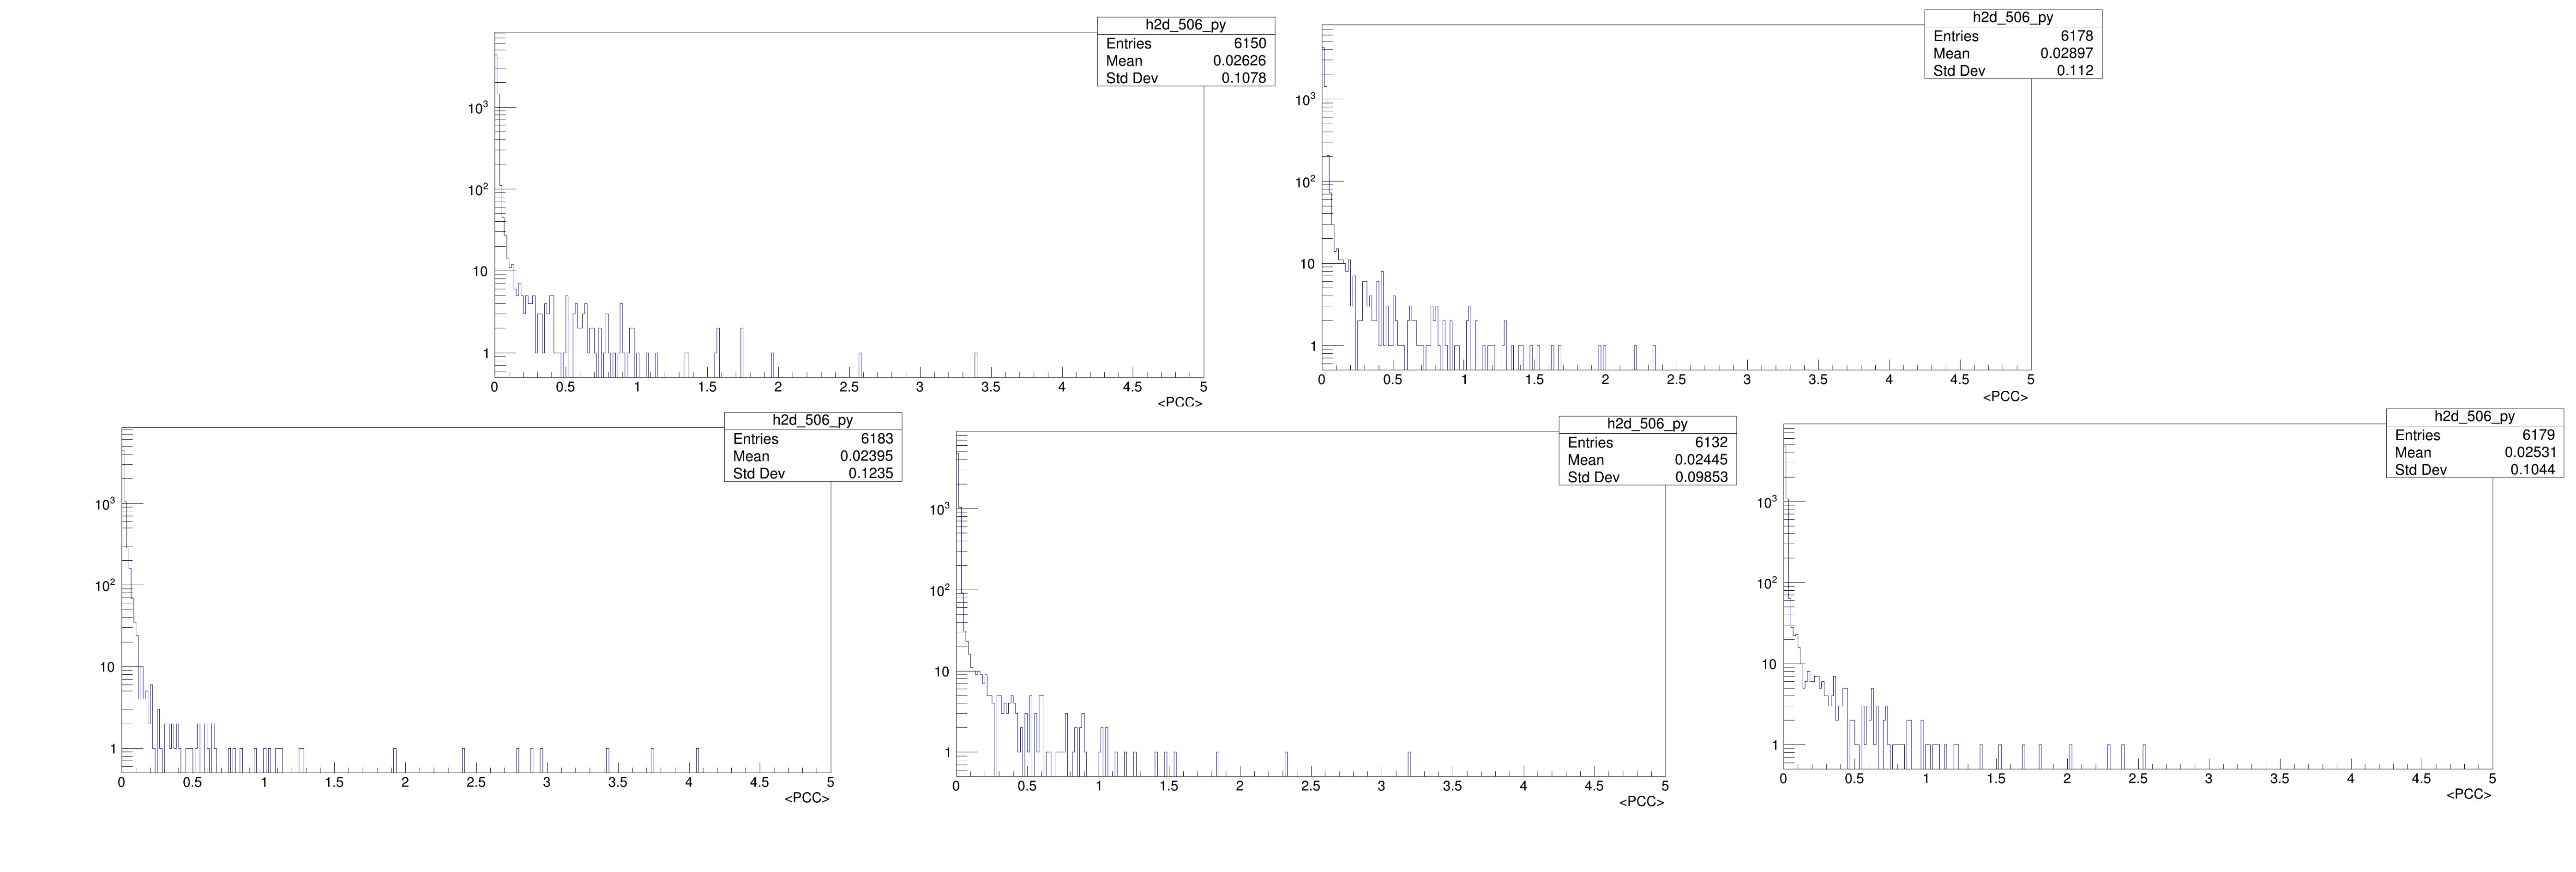
\includegraphics[height=0.4\textheight, width=0.8\textwidth]{sshist.png}
    \caption{Distribution of average PCC for bcid 345 during SS number 2. The PCC values are computed in NB4 time intervals.}
    \label{fig:SShist}
\end{figure}


The mean value during this period is assumed to be the background noise value of this SS period, in the following table we see the mean PCC value for all of the bcids and how it changes in each of the five super separation periods.

\begin{figure}[H]
    \centering
    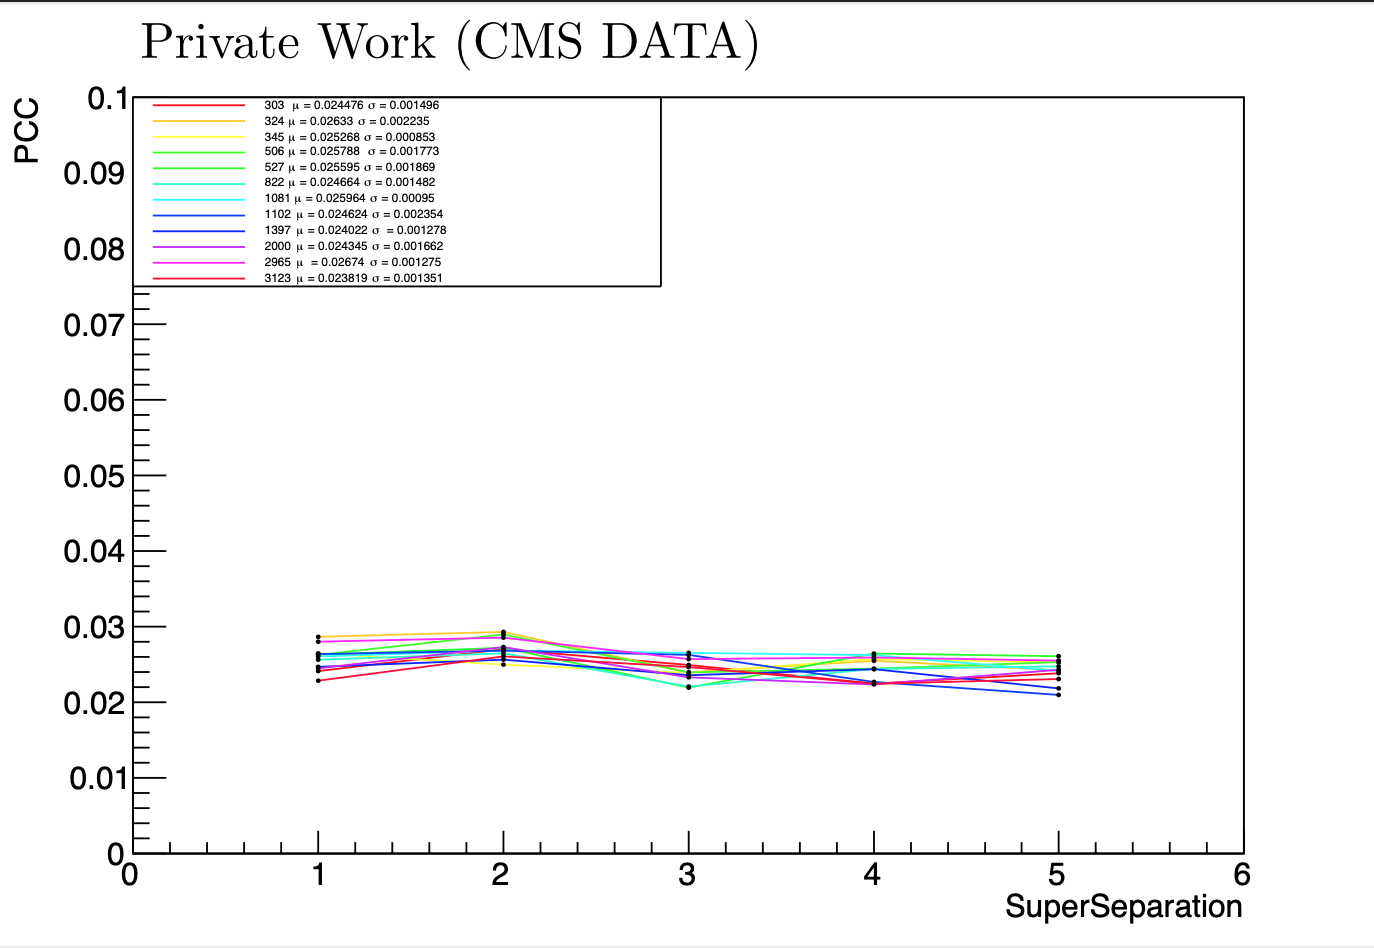
\includegraphics[width=1\textwidth]{SSmean.png}
    \caption{This plot shows the evolution of the PCC value for the twelve differents bcids during the SS periods, it also shows the mean of each bcid.}
    \label{fig:SSmean}
\end{figure}

In principle this value is a single value so we obtain a histogram obtaining a mean for all the mean values for all the 60 values as It's shown on figure (3.6)


\begin{figure}[H]
    \centering
    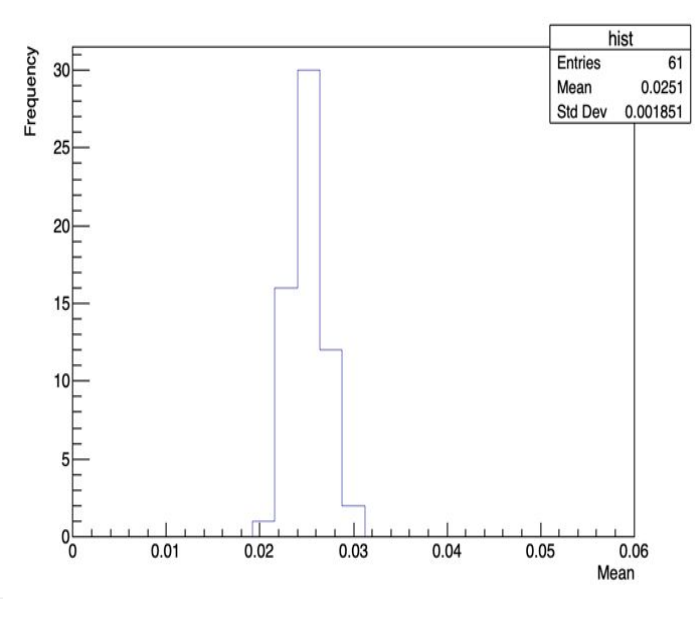
\includegraphics[height = 0.45 \textwidth ,width=1\textwidth]{ssthist.png}
    \caption{This plots shows an histogram with all SS values for all bcids, the mean of all this values is used as the final result.}
    \label{fig:Histogram}
\end{figure}

With this it was obtained that the value for super separation is $ss_{background}$ = 0.0251 +-0.0018 this value will be removed from the PCC rates during the fit for the vdm scans. 

\section{Corrections}

A few corrections were taken into consideration to eliminate noise data from another sources during this vdm calibration, this corrections are applied by the vdM framework. 

\begin{itemize}
  \item \textbf{Background} The rates substracted on the SS periods and is associated with the luminometer itself see section (3.x) for more.
  \item \textbf {Ghost Satellite} This correction have to be with the charge that comes from the non colliding bunches, which are called ghost and those who are leaking from the main radio frequency bucket into another bucket which are called satellite. This currents have an effect on the $\sigma_{visible}$ measure because of the contribution on the charges, this charges are substracted from the beam currents.  \cite{ghost}
  \item \textbf{BeamBeam} This are deflections that happen between bunch crossings, accounting for the electrical repulsion of the beams which increases the lateral separation.   \cite{beambeam}
  \item \textbf{Dynamic beta} This correction accounts for any changes in the proton density distributions of the bunches due to the single particle interaction, resulting into a non linear change during separation steps in transverse bunch profiles and can be described as the effective changes of a called $\beta$ value. \cite{LHClum}
\end{itemize}


\section{Fit model} 

There are different fit models at the time to do the vdm calibration, the most common one is Single Gaussian but also other models like the Double Gaussian, QG, Poly2G or Poly4G. Each of these models have different parameters and restrictions making some of them better than other on the fit quality. 

For the nominal calibration we used the QG fit model this fit model uses the parameter $\beta$, the peak value which is the maximum rate obtained during the head on period, the mean and a q values which is also a parameter. This fit model is given by the following equation:


\begin{equation}
f_{qg}(\Delta x) = peak * e_{q}(-\beta(\Delta x - mean)^{2},q)
\end{equation}

with $e_{q}$ being a function of x defined as: 

\begin{equation}
e_{q}(x, q) = (1+(1-q)x)^{\frac{1}{1-q}}
\end{equation}

This fit model were applied to the data using vdM famework software for all bcids, the figure (3.7) shows this fit on the x plane and on the y plane for one bcid. Other bcids showed a similar result.

\begin{figure}[H]
    \centering
    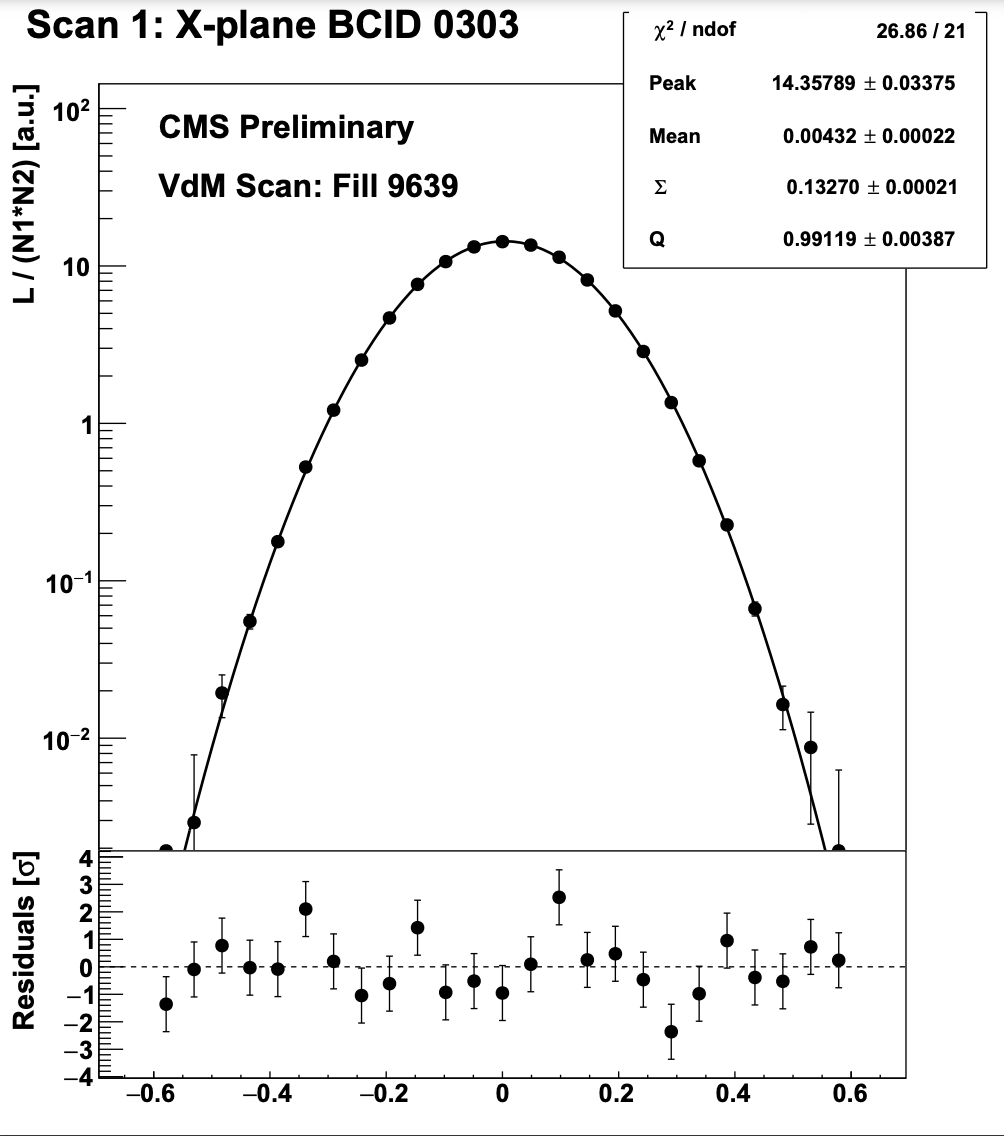
\includegraphics[width=0.45\textwidth]{fitqg1.png}
    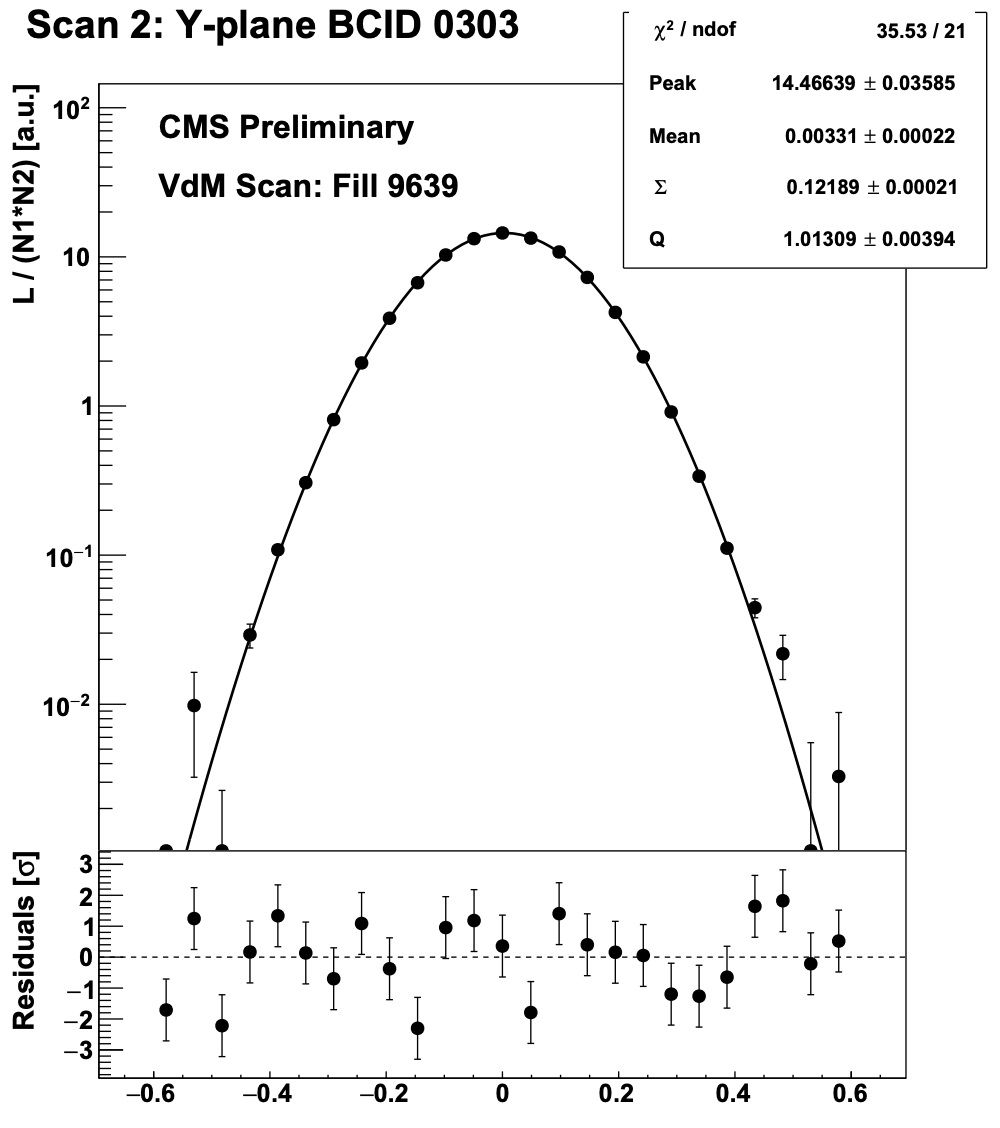
\includegraphics[width=0.45\textwidth]{fitqg2.png}
    \caption{QG Fit on X plane and Y plane}
    \label{fig:QGfit}
\end{figure}

To see if the fit converged we check the status of the covariance matrix if this value is 3 the fit is converged as we can see in the figure (3.8) shows all of the bcids converged in all of the scans for the vdm and BI. 
\begin{figure}[H]
    \centering
    \includegraphics[width=0.9\textwidth]{QG_covStatus.png}
    \caption{Status of the covariance matrix gives 3 for all values showing that all bcids converged with the fit}
    \label{fig:QGfit}
\end{figure}

Also to see the fit quality we obtain the value of $\chi^{2}$ divided by the numbers of degree freedom this graphic is shown on the figure (3.9).

\begin{figure}[H]
    \centering
    \includegraphics[width=0.9\textwidth]{QG_chi2.png}
    \caption{Chi2 values to see the fit quality, the green line represent the mean}
    \label{fig:QGchi2}
\end{figure}

\section{Fit model optimization}

Two fit models were used for this, the first one described above and the second Poly2G. The poly2G model consist on a value r2 which is a parameter, the value $\Sigma$ related to the beam width, the peak which is the maximum rate during the head on period and the mean. Its defined as: 

\begin{equation}
f_{Poly2G}(\Delta x) = peak * ( 1 + r_2 \left( \frac{x - mean}{\sigma / (1 + r_2)} \right)^2 \right) \exp\left( -\frac{1}{2} \left( \frac{x - mean}{\sigma / (1 + r_2)} \right)^2 \right)
\end{equation}

Once the Poly2G fit model was used the chi2 value was compared with the nominal fit model, in the figure (3.9) we can see the chi2 values for each scan. The mean value of the chi2 is lower than the QG that's the reason we used it as the nominal fit model. 

\begin{figure}[H]
    \centering
    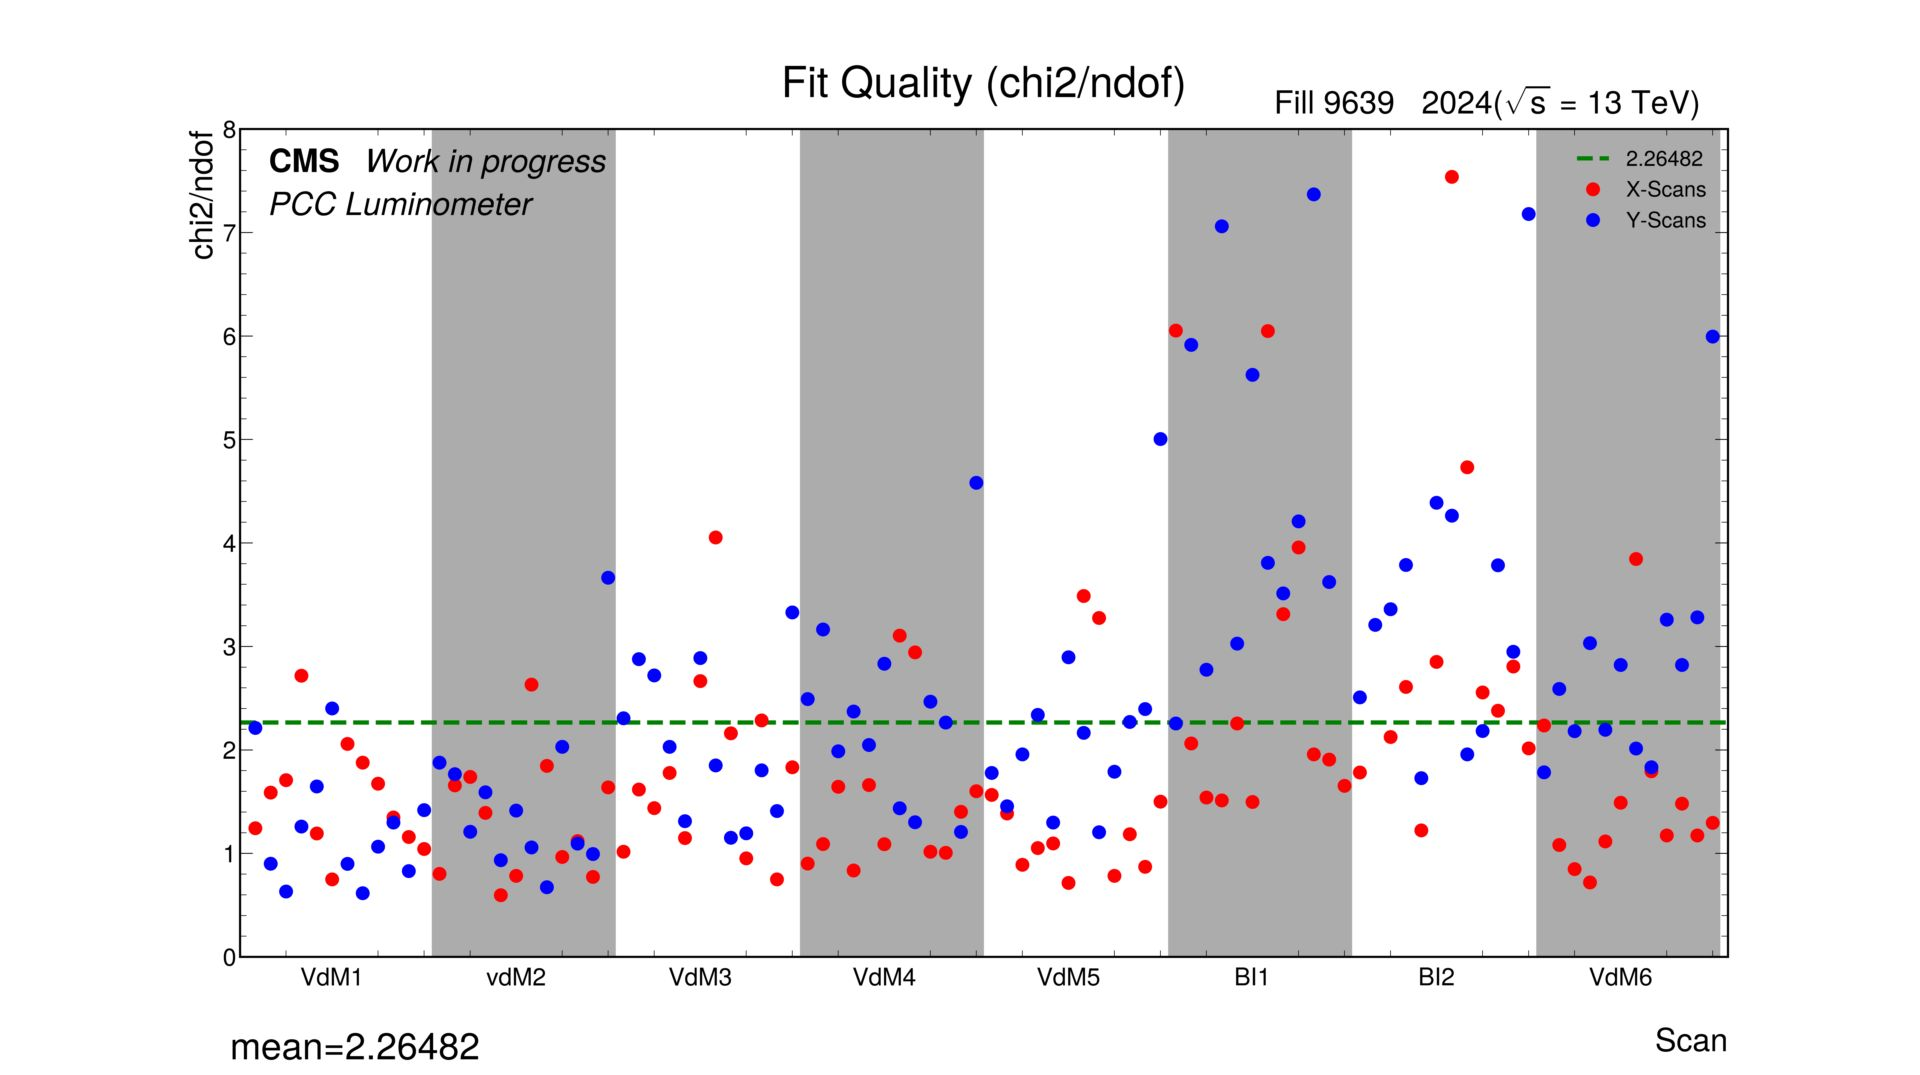
\includegraphics[width=0.9\textwidth]{poly2g.jpeg}
    \caption{Chi2 values to see the fit quality of the poly2g fit model the green line represent the mean, notice that the mean is lower than with the nominal fit model.}
    \label{fig:QGchi2}
\end{figure}

\section{Beam Parameters}

The beam parameters of the vdm scan were obtained after the vdM framework run whit the QG fit model one of the parameters obtained is the peak value, figure 3.12 shows the peak values obtained with the fits to the different vdM scans.

\begin{figure}[H]
    \centering
    \includegraphics[width=0.9\textwidth]{QG_peak.png}
    \caption{QG model fit peak values obtained for the different scans in X and Y.}
    \label{fig:QGpeak}
\end{figure}

Here we can see that the peak values are increasing with the time in the fill, this behavior is then explained if we observe the results for the $\Sigma_{x, y}$ shown in the figure (3.13). Here we see that the $\Sigma_{x, y}$ values are decreasing for each scan reducing the thickness of the beams and thus observing a higher peak value even if the number of particles is decreasing through time. 

\begin{figure}[H]
    \centering
    \includegraphics[width=0.9\textwidth]{QG_CapSigma.png}
    \caption{QG model fit $\Sigma$ values obtained for the different scans in X and Y in the vdM fill.}
    \label{fig:QGcapsigma}
\end{figure}

\section{Results}

After the obtention of the beam parameters  the value of $\sigma_{visible}$ can be obtained, the values for each bcid is shown are shown on the image (3.13).

\begin{figure}[H]
    \centering
    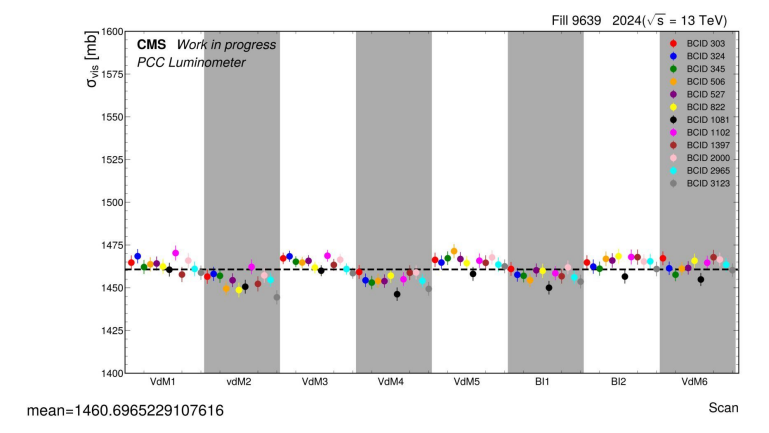
\includegraphics[width=0.9\textwidth]{sigbcid.png}
    \caption{The value of $\sigma_{visible}$ of all twelve bcids and the seven used scans}
    \label{fig:sigbcid}
\end{figure}

We are expecting a constant value of $\sigma_{visible}$ here it appears to be changing each scan this could be to other uncertainties. Then in the image (3.14) Its shown the result on each scan for the weighted mean which is a mean taken into consideration a value mean that is defined as:

\begin{equation}
w_{i}=\frac{1}{\sigma^{2}}
\end{equation}

So then the weighted mean value of $\sigma_{visible}$ would be:

\begin{equation}
\sigma_{vis} = \frac {\Sigma_{i} w_{i} \sigma^{i}_{vis}}{\Sigma_{i} w_{i}} 
\end{equation}

With the error defined as:

\begin{equation}
\sigma_{visErr} = \frac{1}{\sqrt{\Sigma_{i} w_{i}}}
\end{equation}

\begin{figure}[H]
    \centering
    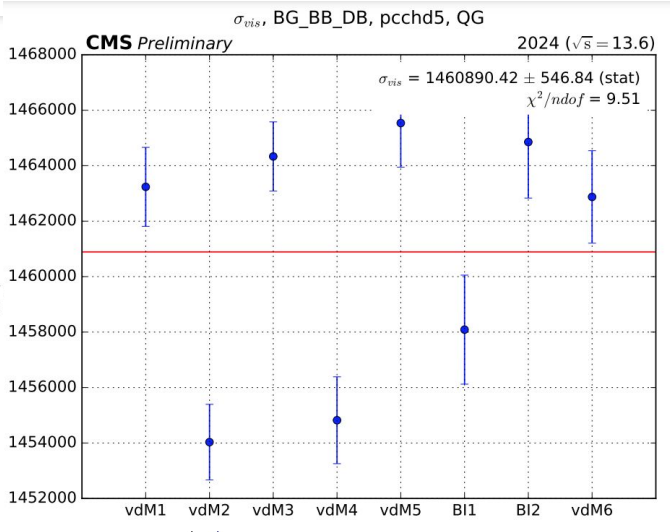
\includegraphics[width=0.9\textwidth]{sigscan.png}
    \caption{$\sigma_{visible}$ weighted mean per each scan}
    \label{fig:sigscan}
\end{figure}

Which give us a $\sigma_{visible}$ value of 

\begin{equation}
\sigma_{visible} = 1460890 \pm 546
\end{equation}

Which is the value for $\sigma_{vis}$ that we have been looking for the calibration using the vdm scans.

The uncertainties from systematics are also taken into consideration, the uncertainties taken in consideration are the one from Background noise, the one from Scan to scan variation and the bunch to bunch variation.

Starting for the Background there were analysis made with the QG model fit which doesn't extract the background PCC, the sigma visible obtained in this case was of $\sigma_{visnobg}$ = 1452589 compared to the value that we obtained $\sigma_{vis}$ = 1450890 can be concluded that the uncertainty is 0.11\%.

In the case of scan to scan variation the standard deviation of the seven scans is taken as uncertainty with a value of 0.30\%. 

For the bunch to bunch uncertainty the value of $\sigma_{vis}$ was obtained on each scan to each value there is a standard deviation assigned which is divided by the mean of the twelve BCIDS. This value is then divided by the square root of the number of bunches, all of this results are show in in the table (3.2). The uncertainty value was 0.02\%.

\begin{table} [H]
\begin{center}
\caption{Bunch to bunch uncertainty table.}
\begin{tabular}{|c c c c|} 
 \hline
 Scan & \sigma_{vis} & STD & Syst. Error  \\ [0.5ex] 
 \hline\hline
 vdM1 & 1463330 & 1220 & 0.02  \\ 
 \hline
 vdM2 & 1453795 & 1212 & 0.02 \\
 \hline
 vdM3 & 1464237 & 953 & 0.01 \\
 \hline
 vdM4 & 1454363 & 1170 & 0.02 \\
 \hline
 vdM5 & 1465271 & 1200 & 0.02  \\ 
 \hline
 BI1 & 1457208 & 1169 & 0.02 \\ 
 \hline
 BI2 & 1464367 & 1233 & 0.02\\
 \hline
 vdM6 &1462515  & 1155 & 0.02 \\ 
 \hline
    \textbf{mean}        &             &            & 0.2 \\ [1.0ex]
 \hline
\end{tabular}
\end{center}
\end{table}

The sum between all the uncertainties can be see in detail in the table (3.3), the total systematic uncertainty is 0.43\% (6281) taking into consideration only those systematic uncertainties. 

\begin{table} [H]
\begin{center}
\caption{Systematic uncertainties total.}
\begin{tabular}{|c c|} 
 \hline
 Systematic  & Systematic uncertainty \\ [0.5ex] 
 \hline\hline
 Background & 0.11\%   \\ 
 \hline
 Bunch to Bunch & 0.02\%  \\
 \hline
 Scan to scan & 0.30\% \\
 \hline
  Total          &     0.43\%  \\ [1.0ex]
 \hline
\end{tabular}
\end{center}
\end{table}

%\begin{table}[H]
%\begin{center}
%\small
%\caption{Comparison of $\sigma_{visible}$ values with different corrections}
%\begin{tabular}{| c| c| c|} 
 %\hline
 %Correction & $\sigma_{visible}$ & Relative Change(\%) \\ [0.5ex] 
 %\hline\hline
% No correction & $1452589 \pm 2041$ & - \\ 
 %\hline
% Background & $1448801 \pm 676$ & +0.26 \\
 %\hline
 %Background + Ghost Satellite & $1450154 \pm 560$ & -0.09 \\
 %\hline
% Background + Ghost Satellite + Beam Beam + Dynamic Beta & $1460890 \pm 546$ & -0.74 \\ [1.0ex]
 %\hline
%\end{tabular}
%\end{center}
%\end{table}
